\documentclass[aspectratio=169, 10pt]{beamer}

% ---------- Tema y colores ----------
\usetheme{default}
\usecolortheme{default}
\setbeamertemplate{navigation symbols}{}
\setbeamertemplate{footline}[frame number]
\setbeamertemplate{frametitle continuation}{}

\definecolor{StanfordRed}{RGB}{140,21,21}
\definecolor{StanfordGray}{RGB}{77,77,77}
\definecolor{LightGray}{RGB}{240,240,240}
\definecolor{AccentBlue}{RGB}{0,84,166}
\definecolor{AccentGreen}{RGB}{0,130,100}
\definecolor{UCMBlue}{RGB}{4, 171, 226}
\definecolor{UCMNavy}{RGB}{20, 65, 134}

% Alias de la paleta antigua: las figuras TikZ de esta clase siguen
% usando mitblue/mitgray, que ahora apuntan a los colores UCM.
\definecolor{mitblue}{RGB}{20, 65, 134}
\definecolor{mitgray}{RGB}{169, 169, 169}
\definecolor{backgroundblue}{HTML}{D7EAF3}
\definecolor{catyellow}{HTML}{FCDA76}
\definecolor{catstripe}{HTML}{F9B74C}
\definecolor{yarnred}{HTML}{E26B6B}
\definecolor{bowlblue}{HTML}{66A3D4}
\definecolor{bboxblue}{HTML}{5E69B1}
\definecolor{bboxred}{HTML}{D9534F}
\definecolor{bboxgreen}{HTML}{008000}

\setbeamercolor{frametitle}{fg=white, bg=UCMBlue}
\setbeamercolor{title}{fg=white}
\setbeamercolor{author}{fg=white}
\setbeamercolor{institute}{fg=white!80}
\setbeamercolor{structure}{fg=UCMBlue}
\setbeamercolor{block title}{bg=UCMBlue!15!white, fg=UCMBlue}
\setbeamercolor{block body}{bg=LightGray}
\setbeamercolor{block title alerted}{bg=StanfordRed!15!white, fg=StanfordRed}
\setbeamercolor{block body alerted}{bg=LightGray}
\setbeamercolor{block title example}{bg=AccentGreen!15!white, fg=AccentGreen}
\setbeamercolor{block body example}{bg=LightGray}
\setbeamercolor{alerted text}{fg=UCMBlue}
\setbeamercolor{example text}{fg=UCMBlue}

\setbeamerfont{frametitle}{series=\bfseries, size=\large}
\setbeamerfont{title}{series=\bfseries, size=\LARGE}
\setbeamerfont{block title}{series=\bfseries}

% ---------- Paquetes ----------
\usepackage[utf8]{inputenc}
\usepackage[T1]{fontenc}
\usepackage[provide=*,spanish]{babel}
\usepackage{amsmath, amssymb, bm}
\usepackage{graphicx}
\usepackage{tikz}
\usepackage{pgfplots}
\pgfplotsset{compat=1.18}
\usetikzlibrary{arrows, arrows.meta, shapes, shapes.geometric, positioning,
	fit, calc, matrix, chains, mindmap, decorations.pathreplacing,
	backgrounds, shadows, patterns}
\usepackage{booktabs}
\usepackage{xcolor}
\usepackage{multicol}
\usepackage{tcolorbox}
\tcbuselibrary{skins, breakable}
\usepackage{import}
\subimport{./layers/}{init}
\usepackage{tikzlings}
\usepackage{neuralnetwork}


% ---------- Comandos útiles ----------
\providecommand{\R}{\mathbb{R}}
\providecommand{\E}{\mathbb{E}}
\providecommand{\Var}{\operatorname{Var}}
\providecommand{\relu}{\operatorname{ReLU}}

\newcommand{\formula}[1]{%
	\begin{tcolorbox}[colback=UCMBlue!8, colframe=UCMBlue, arc=4pt,
		boxsep=2pt, left=6pt, right=6pt, top=3pt, bottom=3pt]
		#1
	\end{tcolorbox}
}

% ---------- Portada ----------
\title{\textbf{Modelos Generativos}}
\subtitle{Autoencoders variacionales y modelos de flujo}
\author{Sergio Hern\'andez, PhD\\ shernandez@ucm.cl}
\institute{
	\begin{tikzpicture}[scale=0.42, every node/.style={transform shape}]
		\foreach \i/\y in {1/0,2/1,3/2}{\node[circle,draw=white,fill=white!20,minimum size=4mm] (i\i) at (0,\y){};}
		\foreach \i/\y in {1/-0.5,2/0.5,3/1.5,4/2.5}{\node[circle,draw=white,fill=white!35,minimum size=4mm] (h\i) at (2,\y){};}
		\foreach \i/\y in {1/0.5,2/1.5}{\node[circle,draw=white,fill=white!50,minimum size=4mm] (o\i) at (4,\y){};}
		\foreach \a in {1,2,3}\foreach \b in {1,2,3,4}{\draw[white,opacity=0.5] (i\a)--(h\b);}
		\foreach \a in {1,2,3,4}\foreach \b in {1,2}{\draw[white,opacity=0.5] (h\a)--(o\b);}
	\end{tikzpicture}
	\\ \textbf{Mag\'ister en Data Science --- Universidad Cat\'olica del Maule}}
\date{}


\begin{document}
% --- Título ---
{
	\setbeamertemplate{background}{
		\begin{tikzpicture}[remember picture, overlay]
			\fill[UCMBlue] (current page.south west) rectangle (current page.north east);
			\fill[UCMBlue!70!black, opacity=0.5]
			(current page.south west) -- ++(0,3) -- ++(18,0) -- cycle;
			\foreach \i in {1,...,40}{
				\fill[white, opacity=0.04]
				({random()*17}, {random()*10}) circle ({random()*0.3});
			}
		\end{tikzpicture}
	}
	\begin{frame}[plain]
		\vspace{1.2cm}
		\titlepage
		\begin{tikzpicture}[remember picture, overlay]
			\node[white, opacity=0.15, font=\fontsize{80}{80}\selectfont]
			at (current page.east) [xshift=-2cm] {$p_\theta$};
		\end{tikzpicture}
	\end{frame}
}

\section{Introducci\'on}
% --- Diapositiva 1: Introducción ---
% =================================================================
% SECCIÓN 1: OPTIMIZACIÓN
\begin{frame}{Introducción: IA Generativa}
	\begin{columns}
		\begin{column}{0.4\textwidth}
			\begin{itemize}
				\item Una nueva generación de sistemas de IA capaces de crear contenido nuevo.
				\item Ejemplos:
				\begin{itemize}
					\item Generación de texto (borradores, resúmenes).
					\item Creación de imágenes artísticas.
					\item Producción de videos realistas.
				\end{itemize}
			
			\end{itemize}
		\end{column}
		\begin{column}{0.6\textwidth}
			\begin{figure}
			\begin{center}
				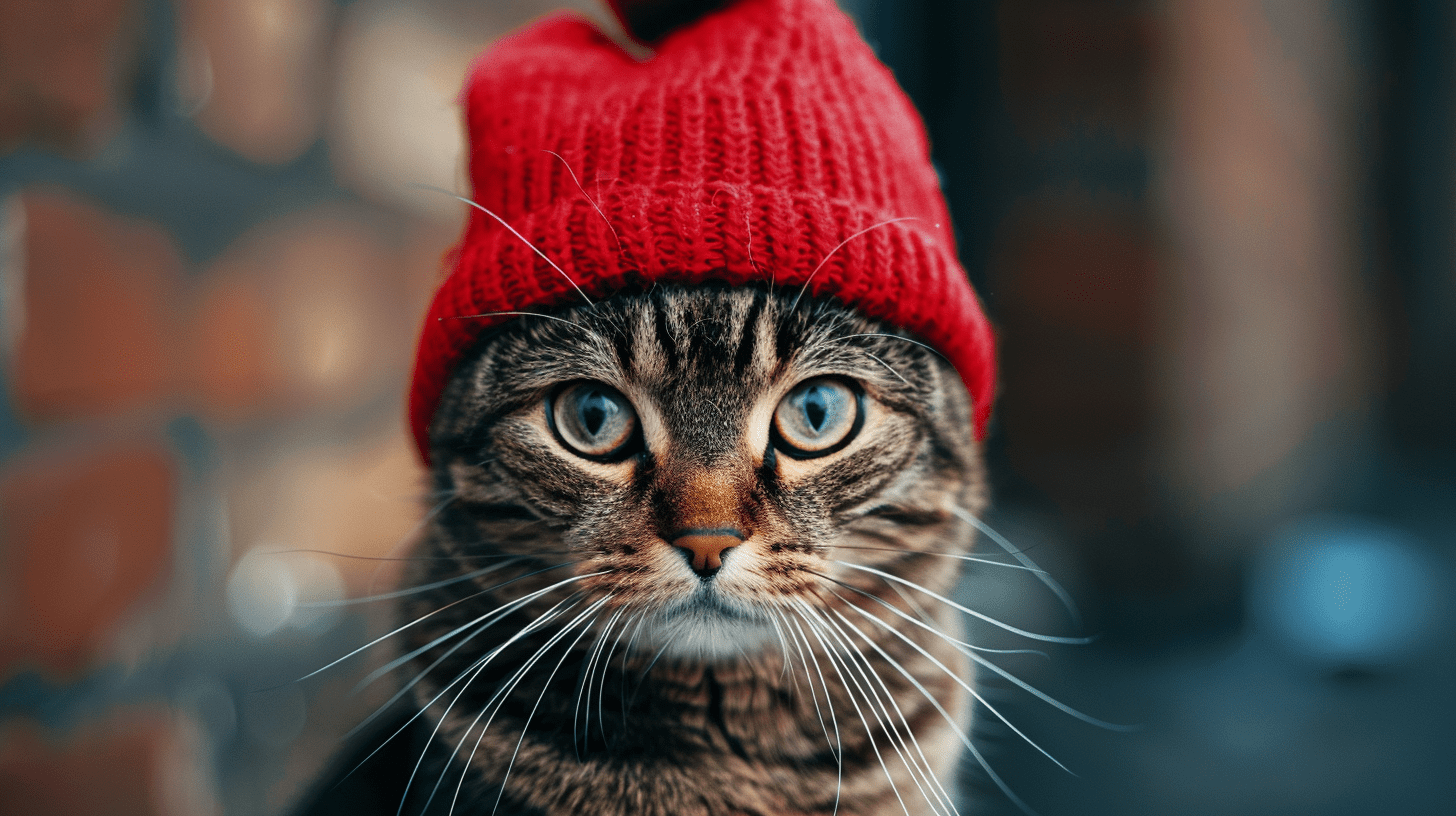
\includegraphics[scale=0.15]{figures/generative_ai}
				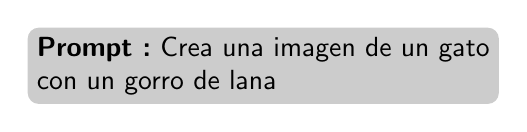
\begin{tikzpicture}
					%\node[font=\scriptsize\bfseries] at (-1,0){Prompt : Crea una imagen de un gato con un gorro de lana};
					\node[fill = gray!40, shape = rectangle, rounded corners,
					minimum width = 4cm, font = \sffamily,align=left] {\textbf{Prompt :} Crea una imagen de un gato\\ con un gorro de lana}; 
				\end{tikzpicture}
			\end{center}
				%\caption{Ejemplos de IA Generativa}
			\end{figure}
		\end{column}
	\end{columns}
\end{frame}

\begin{frame}{Modelos Generativos}
	
	
	\begin{columns}[T]
		\begin{column}{0.5\textwidth}
			\begin{block}{modelos generativos}		
				\begin{itemize}
					\item Los modelos de clasificación mapean imágenes a etiquetas $f:\mathcal X \mapsto \mathcal Y$. Esta es una relación muchos a uno.
					\item Los modelos generativos mapean etiquetas a imágenes $g:\mathcal Y \mapsto \mathcal X$. Esta es una relación uno a muchos. Para manejar esta ambiguedad $g$ es una función de probabilidad.  
				\end{itemize}
				
			\end{block}
		\end{column}
		
		\begin{column}{0.5\textwidth}
			\begin{center}
				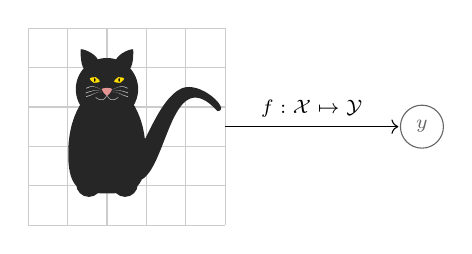
\begin{tikzpicture}[scale=1.0]
					%\draw[step=0.5, red!20] (-0.5,-0.5) grid (3,3);
					\draw[step=0.5, black!20] (0,0) grid (2.5,2.5);
					\cat[xshift=1.0cm,yshift=0.25cm,scale=0.9];
					\draw[->] (2.5,1.25) -- (4.7,1.25) node[midway,sloped,above,font=\scriptsize] {$f:\mathcal X \mapsto \mathcal Y$};
					\node[draw,shape=circle,font=\scriptsize, black!60] at (5, 1.25) {$y$};
				\end{tikzpicture}
				\\
				\vspace{1.0cm}
				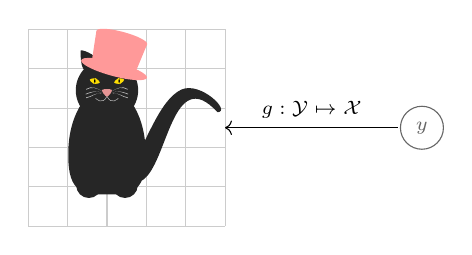
\begin{tikzpicture}[scale=1.0]
					%\draw[step=0.5, red!20] (-0.5,-0.5) grid (3,3);
					\draw[step=0.5, black!20] (0,0) grid (2.5,2.5);
					\cat[xshift=1.0cm,yshift=0.25cm,scale=0.9,tophat=red!40];
					\draw[<-] (2.5,1.25) -- (4.7,1.25) node[midway,sloped,above,font=\scriptsize] {$g:\mathcal Y \mapsto \mathcal X$};
					\node[draw,shape=circle,font=\scriptsize, black!60] at (5, 1.25) {$y$};
				\end{tikzpicture}
			\end{center}
		\end{column}
	\end{columns}
\end{frame}


\begin{frame}{Distribuciones Estructuradas}
	\begin{block}{Redes Bayesianas (Kim \& Pearl 1983, Pearl 1988)}		
		\begin{itemize}
			\item Utilizan un modelo gráfico (grafo) para representar una distribución conjunta entre variables aleatorias. 
			\item Induce una relación de independencia condicional $p(a,b,c)=p(c|a,b)p(b|a)p(a)$
		\end{itemize}
		\begin{figure}
			\tikzstyle{max}=[draw,thick,circle,minimum size=15pt,inner sep=0pt]
			\tikzstyle{selected vertex} = [vertex, fill=red!24]
			\tikzstyle{edge} = [draw,thick,->]
			\tikzstyle{weight} = [font=\small]
			\begin{tikzpicture}[scale=.8, auto,swap]
				\foreach \pos/\name/\weight in { {(0,0)/A/a}, {(2,0)/B/b},{(1,-1)/C/c}}
				\node[max] (\name) at \pos {$\weight$};
				% Connect vertices with edges and draw weights
				\foreach \source/ \dest /\weight in {A/B,A/C,B/C}
				\path[edge] (\source) -- node[weight] {} (\dest);        
			\end{tikzpicture}
		\end{figure}
	\end{block}
	\pause
	\begin{itemize}
	\item Las Redes Bayesianas permiten calcular la probabilidad de un evento dada la evidencia.  
	\item Son ampliamente usadas en modelos causales y en entornos donde se requiere explicar las predicciones (diagnóstico médico, sistema de apoyo  a las decisiones, visión computacional). 
\end{itemize}
\end{frame}


\begin{frame}[shrink]{Teorema de Bayes}
	
	\begin{block}{Teorema de Bayes}
		\begin{align*}
			\underbrace{\text{posterior}}_{P(B \vert A)}&=\frac{\underbrace{\text{verosimilitud}}_{P(A \vert B)} \times \underbrace{\text{prior}}_{P(B)}}{\underbrace{\text{evidencia}}_{P(A)}}\\
		\end{align*} 
	\end{block}
	\begin{columns}
		\begin{column}{0.5\textwidth}
			\begin{align*}
				\mathbf{z} &\in \{\text{Feliz},\text{Enojado}\}\\
				p(\mathbf{z} \vert \mathbf{x})&=\frac{p(\mathbf{x} \vert  \mathbf{z}) \times  p(\mathbf{z})}{p(\mathbf{x})}
			\end{align*}
		\end{column}
	
		\begin{column}{0.5\textwidth}
			\begin{center}
					\tikzstyle{max}=[draw,thick,fill=bboxred!60,circle,minimum size=10pt,inner sep=0pt,font=\scriptsize]
					\tikzstyle{min}=[draw,thick,circle,minimum size=10pt,inner sep=0pt,font=\scriptsize]

				\tikzstyle{edge} = [draw,->,bboxred!60]
				\begin{tikzpicture}[scale=1.4]
				        \draw[rounded corners,mitgray] (1.0,0.0) -- (1.0,2.7) -- (3.5,2.7) -- (3.5,0.0) -- (1.,0.0) ;
					%\draw[step=0.5, red!20] (-0.5,-0.5) grid (3,3);
					%\draw[step=0.5, black!20] (0,0) grid (3.5,3.5);
					\cat[xshift=1.75cm,yshift=0.35cm,scale=1];
					\foreach \pos/\name/\weight in { {(1.75,2)/A/$x_1$}, {(1.75,1.5)/B/$x_2$},{(1.75,0.8)/C/$x_5$},{(1.5,1.3)/D/$x_3$},{(2,1.3)/E/$x_4$},{(1.5,0.6)/F/$x_6$},{(2,0.6)/G/$x_7$}}
					\node[max] (\name) at \pos {\weight};
					\foreach \source/ \dest  in {B/A,B/C,B/D,B/E,C/F,C/G}
					\path[edge] (\source) -- (\dest);
					\node[min]  at (4.25, 1.25) {$\mathbf{z}$}; 
					\path[draw,<-,mitgray] (3.5,1.25) -- (4.10,1.25);
					\end{tikzpicture}
			\end{center}
		\end{column}
	\end{columns}


\end{frame}

\begin{frame}{Inferencia}
	
	\begin{block}{Inferencia Bayesiana}
		\begin{itemize}
			\item La tarea b\'asica del m\'etodo de inferencia probabilistico es calcular la distribuci\'on posterior para un nodo dado que se conoce el valor de un conjunto de nodos que aportan evidencia.
			\item En el caso de la estructuras de grafos en serie (cadenas), el proceso de inferencia requiere aplicar de manera repetida el teorema de Bayes.
		\end{itemize}
	\end{block}

\tikzstyle{max}=[draw,circle,minimum size=20pt,inner sep=0pt]
\tikzstyle{selected vertex} = [vertex, fill=red!24]
\tikzstyle{edge} = [draw,thick,->]
\tikzstyle{weight} = [font=\small]
\begin{figure}
	\begin{tikzpicture}[scale=1, auto,swap]
		\foreach \pos/\name/\weight in { {(0,0)/A/$x_1$}, {(2,0)/B/$x_2$}, {(4,0)/C/$x_3$},{(6,0)/D/$x_4$}}
		\node[max] (\name) at \pos {\weight};
		% Connect vertices with edges and draw weights
		\foreach \source/ \dest /\weight in {A/B,B/C,C/D}
		\path[edge] (\source) -- node[weight] {} (\dest);   
		\node[fill = gray!40, shape = rectangle, rounded corners,
		minimum width = 4cm, font = \sffamily\bf,align=left] at (2.0, -1.25) {El cielo es }; 
		\node[fill = red!40, shape = rectangle, rounded corners,
		minimum width = 2cm, font = \sffamily\bf,align=left] at (6.0, -1.25) {azul};      
	\end{tikzpicture}
\end{figure}	
\begin{align}
p_\theta(\mathbf{x}) = \prod_{i=1}^{N} p_\theta(x_i \vert \mathbf{x}_{<i})
\end{align}
\end{frame}

\begin{frame}[shrink]{Autoencoders Variacionales}
	\begin{block}{VAE (Kingma \& Welling, 2011)}		
		\begin{itemize}
			\item Los Autoencoders utilizan una variable latente $\mathbf z$ y una distribución marginal $p(\mathbf{x})= \int p_\theta(\mathbf{x} \vert  \mathbf{z}) p( \mathbf{z}) \text{d}\mathbf{z}$
			\item El modelo generativo utiliza una distribución apriori $z \sim p(\mathbf z)$ y luego genera muestras de acuerdo a $\mathbf{x} \sim p(\mathbf{x})$
			\item Dado que obtener muestras directamente desde $p(\mathbf{x})$ es intratable, el modelo VAE utiliza una cota inferior de la verosimilitud $q_\theta(z \vert x)$.
	\end{itemize}
		
	\end{block}
	\begin{figure}
		\centering
		\resizebox{0.5\textwidth}{!}{%
	\begin{tikzpicture}
\tikzstyle{connection}=[ultra thick,every node/.style={sloped,allow upside down},draw=gray,opacity=0.7]
\tikzstyle{copyconnection}=[ultra thick,every node/.style={sloped,allow upside down},draw={rgb:blue,4;red,1;green,1;black,3},opacity=0.7]
\pic[shift={(0,0,0)}] at (0,0,0) 
    {Box={
        name=conv0,
        caption= ,
        %xlabel={{1, }},
        %zlabel=32,
        fill=mitblue!50,
        height=32,
        width=1,
        depth=32
        }
    };


\pic[shift={(1,0,0)}] at (conv0-east) 
    {Box={
        name=conv1,
        caption= ,
        %xlabel={{6, }},
        %zlabel=28,
        fill=mitblue!50,
        height=28,
        width=6,
        depth=28
        }
    };


%\draw [connection]  (conv0-east)    -- node {\midarrow} (conv1-west);


\pic[shift={ (2,0,0) }] at (conv0-east) 
    {Box={
        name=pool1,
        caption=$q_\theta(z \vert x)$ ,
        fill=red!20,
        opacity=0.5,
        height=14,
        width=6,
        depth=14
        }
    };


\pic[shift={(1,0,0)}] at (pool1-east) 
    {Box={
        name=latent,
        caption=$z$ ,
        %xlabel={{16, }},
        %zlabel=10,
        fill=mitblue!50,
        height=10,
        width=16,
        depth=10
        }
    };

\pic[shift={ (1,0,0) }] at (latent-east) 
    {Box={
        name=pool2,
        caption=$p_\theta(x \vert z)$ ,
        fill=red!20,
        opacity=0.5,
        height=14,
        width=6,
        depth=14
        }
    };
   
 \pic[shift={(1,0,0)}] at (pool2-east) 
    {Box={
        name=conv2,
        caption= ,
        %xlabel={{6, }},
        %zlabel=28,
        fill=mitblue!50,
        height=28,
        width=6,
        depth=28
        }
    };

\pic[shift={(1,0,0)}] at (conv2-east) 
    {Box={
        name=conv_gen,
        caption= ,
        %xlabel={{1, }},
        %zlabel=32,
        fill=mitblue!50,
        height=32,
        width=1,
        depth=32
        }
    };
\end{tikzpicture}%
		} % Fin de resizebox
	\end{figure}

\end{frame}


\begin{frame}{Modelos de Flujo}
	\begin{block}{Flujo Normalizador (Rezende \& Mohamed, 2015)}		
		\begin{itemize}
			\item Es un modelo que utiliza redes neuronales para aprender distribuciones complejas a partir de transformaciones de distribuciones mas simples.
			\item Permiten obtener muestras de distribuciones complejas y a la vez evaluar la probabilidad de observar nuevos ejemplos.
			\item Se basa en el terorema de cambio de variables a partir de transformaciones invertibles $\phi^{-1}$
		\end{itemize}
		
	\end{block}

\begin{figure}
	\centering
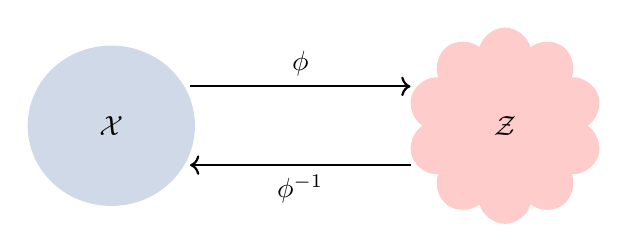
\begin{tikzpicture}[decoration=zigzag]
	\node at (1.5,1) [inner sep=6mm,fill=mitblue!20,ellipse] {$\mathcal X$};
	\node at (6.5,1) [inner sep=6mm,fill=red!20,cloud] {$\mathcal Z$};
	\path[draw,thick,->] (2.5,1.5) -- node[above] {$\phi$} (5.3,1.5); 
	\path[draw,thick,<-] (2.5,0.5) -- node[below] {$\phi^{-1}$} (5.3,0.5); 
\end{tikzpicture}
\end{figure}
		
\end{frame}


\begin{frame}{Cambio de Variables}
	\begin{block}{Conservación de Masa}		
		
			\begin{align*}
			\int_{\mathcal X} p(\mathbf{x}) d\mathbf{x}= \int_{\mathcal Z} p(\mathbf{z}) d\mathbf{z}=1
			\end{align*}
	
		
	\end{block}

\begin{columns}[T]
	\begin{column}{0.5\textwidth}
	\begin{align*}
		p(\mathbf{z}) = p(\mathbf{x}) \left\vert \text{det}\left(\frac{\partial \phi(\mathbf{x})}{\partial \mathbf{x}}\right) \right\vert ^{-1}
	\end{align*}
	\end{column}
	
	\begin{column}{0.5\textwidth}
	\begin{align*}
		\phi(x)&=\log(x-a)\\
		\phi^{-1}(z)&=\exp(z)+a\\
		p(z)&=p(x)\left\vert \text{det}\left(\frac{\partial \phi(\mathbf{x})}{\partial \mathbf{x}}\right) \right\vert ^{-1}\\
		&=p(x)\exp(z)
	\end{align*}
	\end{column}
\end{columns}	

	
	
\end{frame}

\begin{frame}{Modelos de Flujo}

		\newcommand{\distro}[4][40]{
			\begin{tikzpicture}[thick]
				%\draw[dashed, dash pattern={on 2.3 off 2}] (0, .4) circle (12mm);
			%	\draw[blue!60!black, very thick] plot[variable=\t, domain=-1:1, samples=#1] ({\t}, {#2 * exp(-10*(\t)^2) + #3 * exp(-60*(\t-0.6)^2 - \t) + #3 * exp(-60*(\t+0.7)^2 - 0.2) + #4 * 0.5 * exp(-50*(\t+0.3)^2) + #4 * exp(-50*(\t-0.2)^2 + 0.1)});
				%\draw[solid, ->] (-1, 0)--(1, 0);
				%\draw[solid, ->] (0, -0.5)--(0, 1.25);
			\end{tikzpicture}
		}
\begin{figure}
	\centering
	\resizebox{\textwidth}{!}{%		
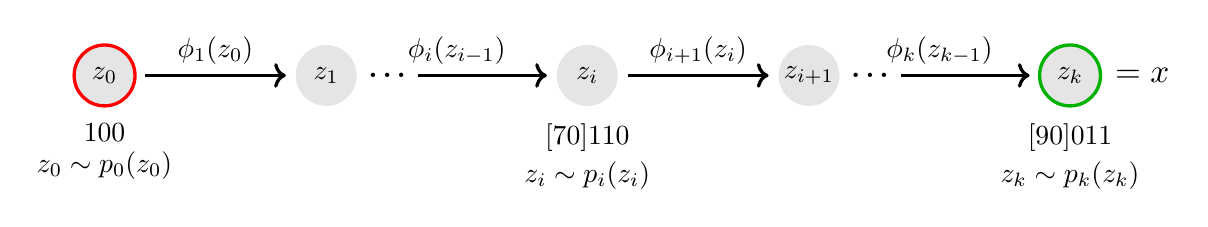
\begin{tikzpicture}[
	node distance=2, very thick,
	flow/.style={shorten >=3, shorten <=3, ->},
	znode/.style={circle, fill=black!10, minimum size=22, inner sep=0}
	]
	
	\node[znode, draw=red] (z0) {$z_0$};
	\node[znode, right=of z0] (z1) {$z_1$};
	\draw[flow] (z0) -- node[above, midway] {$\phi_1(z_0)$} (z1);
	
	\node[znode, right=2.5 of z1] (zi) {$z_i$};
	\node[znode, right=of zi] (zip1) {$z_{i+1}$};
	\draw[flow] (zi) -- node[above, midway] {$\phi_{i+1}(z_i)$} (zip1);
	\draw[flow, shorten <=5ex] (z1) -- node[pos=0.16, inner sep=1] {\textbf\dots} node[above, midway] {$\phi_i(z_{i-1})$} (zi);
	
	\node[znode, draw=green!70!black, right=2.5 of zip1] (zk) {$z_k$};
	\draw[flow, shorten <=5ex] (zip1) -- node[pos=0.16, inner sep=1] {\textbf\dots} node[above, midway] {$\phi_k(z_{k-1})$} (zk);
	\node[right=0 of zk, scale=1.2] {$= x$};
	\node[outer sep=0, inner sep=0, below=0.2 of z0, label={below:$z_0 \sim p_0(z_0)$}] (f0) {\distro{1}{0}{0}};
	\node[outer sep=0, inner sep=0, below=0.2 of zi, label={below:$z_i \sim p_i(z_i)$}] (fi) {\distro[70]{1}{1}{0}};
	\node[outer sep=0, inner sep=0, below=0.2 of zk, label={below:$z_k \sim p_k(z_k)$}] (fk) {\distro[90]{0}{1}{1}};
	
\end{tikzpicture}
%
} % Fin de resizebox
\end{figure}
\begin{itemize}
	\item Inicia generando una variable aleatoria $\mathbf z_0 \sim \mathcal N(0,I¸)$
	\item Realiza $k$ transformaciones biyectivas de manera sucesiva $\phi_k$
	\item Genera muestras $\mathbf x=\mathbf z_k$ al final de la cadena
	
	\begin{align}
		\mathbf x= \phi_k \circ \phi_{k-1} \circ \cdots \circ \phi_1(\mathbf z_0)  
	\end{align}
\end{itemize}
\end{frame}




\end{document}